\begin{frame}{Activité: le jeu de Nim}

  Voici un premier petit jeu simple, pour rentrer dans le sujet.

  \begin{block}{Matériel}
    \begin{itemize}
    \item 16 petits objets (clous, allumettes, boulettes de papier ... peu importe !)
    \end{itemize}
  \end{block}

  \begin{block}{Règle du jeu}
    \begin{itemize}
    \item Disposer les 16 objets sur une table
    \item Les deux joueurs prennent tour à tour 1, 2 ou 3 objets
    \item Le joueur qui prend le dernier objet à gagné
    \end{itemize}
  \end{block}

  \bigskip \bigskip  \bigskip \bigskip

  \begin{center}
    % rendre l'illustration plus utile en la transformant en exemple de partie?
    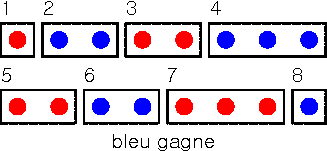
\includegraphics[width=0.8\linewidth]{img/nim.pdf}
  \end{center}

\end{frame}

\begin{frame}{Ce qu'il faut retenir du jeu de Nim}

  \begin{block}{L'intérêt majeur de ce jeu est qu'il est sans suspense 
      {\color{black}\normalsize(voire, sans intérêt ;)}}
    \begin{itemize}
    \item Celui qui commence (\structure{J1}) perd, car il existe un truc pour
      que \structure{J2} gagne à tous les coups
    \item \structure{Stratégie gagnante:} Laisser 4, 8, 12 ou 16 objets à
      l'adversaire (un multiple de 4)
    \end{itemize}
  \end{block}

  \begin{block}{Se convaincre de l'efficacité de la stratégie gagnante}
    Prenons le dernier tour comme exemple. Il reste 4 objets, et J1 joue.

    \begin{columns}
      \begin{column}{.55\linewidth}
        \begin{itemize}
        \item Si J1 prend \alert{1} objet, J2 en prend \structure{3} (dont le dernier) 
        \item Si J1 prend \alert{2} objets, J2 en prend \structure{2} (dont le dernier)
        \item Si J1 prend \alert{3} objets, J2 en prend \structure{1} (le dernier) 
        \end{itemize}        
      \end{column}
      \begin{column}{.45\linewidth}
        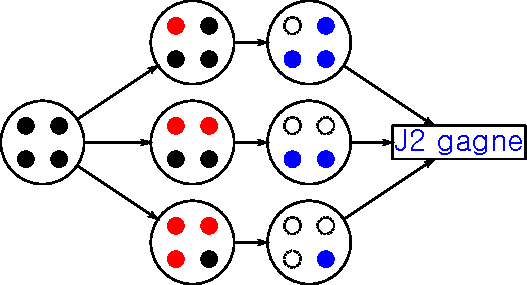
\includegraphics[width=0.8\linewidth]{img/nim4.pdf}
      \end{column}
    \end{columns}

    Dans ce cas, si J2 sait jouer, J1 perd à tous les coups.
    
    En appliquant la même méthode, J2 peut guider le jeu de manière à passer de
    16 objets à 12, puis 8 et enfin 4. Donc, si J2 sait jouer, J1 a perdu la
    partie avant même de commencer.
    
    \center{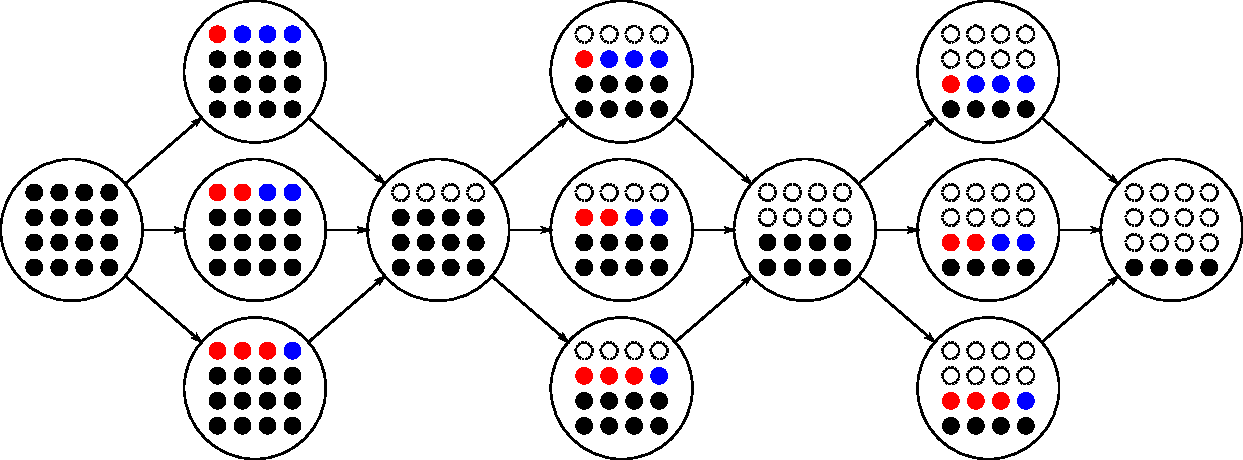
\includegraphics[width=0.8\linewidth]{img/nim16.pdf}}
  \end{block}

  \begin{block}{Le rapport avec l'informatique}
    \begin{itemize}
    \item Passer de la situation initiale à la situation finale à coup sûr demande d'avoir
      une \textit{stratégie gagnante}
    \item C'est un \alert{\textbf{algorithme}} en informatique, une recette de
      cuisine ou un manuel de montage de meubles
    \item Pour se faire obéir du tas de fils, l'informaticien cherche
      l'algorithme pour résoudre le problème,\\
      puis il écrit le \alert{\textbf{programme}} (traduction de l'algorithme
      dans un langage informatique)
    \end{itemize}
  \end{block}

\end{frame}

\begin{frame}

  \begin{block}{pour aller plus loin ...}
    \begin{itemize}
    \item Sous quelle condition est-on sûr de gagner si le nombre de objets n'est
      pas un multiple de 4 ?
    \item Que faudrait-il changer pour gagner à coup sûr si les joueurs ne peuvent
      prendre qu'un ou deux objets à la fois ?
    \end{itemize}
  \end{block}

\end{frame}

%%% Local Variables: 
%%% mode: latex
%%% TeX-master: "CSIRL"
%%% End: 